We show the viability of the microservices approach in Kvik by describing the
MIxT web application for exploring and comparing
transcriptional profiles from blood and tumor samples. 

\subsection*{MIxT Analysis Tasks}

We define six data exploration tasks that the web application should help users
perform: 

\textbf{Explore co-expression gene sets in tumor and blood tissue}. We want to
simplify the process of exploring the computed co-expression gene sets, or
modules, through the web-application. The application should 
visualize gene expression patterns together with clinicopathological variables
for each module. In addition we want to enable users to study the underlying
biological functions of each module by including gene set analyses between the
module genes and known gene sets. 

\textbf{Explore co-expression relationships between genes}. Users should be able
to explore the co-expression relationship as a graph visualization. The network
should visualize each gene as a node and a significant co-expression
relationship as an edge.  

\textbf{Explore relationships between modules from each tissue.} Users should be
able to explore the relationship between modules from different tissues. We
provide two different metrics to compare modules, and the web application should
enable users to interactively browse these relationships. In addition to
providing visualizations the compare modules from each tissue, users should also
be able to explore the relationships, but for different breast cancer patient
groups. 

\textbf{Explore relationships between clinical variables and modules.} In
addition to comparing the association between modules from both tissues, users
also have the possibility of exploring the association with a module and a
specific clinical variable. This should also be possible for the different
breast cancer patient group. 

\textbf{Explore association between user-submitted gene lists and computed
modules.} We want to enable users to explore their own gene lists to explore
them in context of
the co-expression gene sets. The web application must handle uploads of gene
lists and compute association between the genelist and the MIxT modules on
demand. 

\textbf{Search for genes or gene lists of intrest}. To facilitate faster lookup
of genes and biological processes, the web application should provide a search
functionality that lets users locate genes or gene lists and show association to
the co-expression gene sets. 


% LAB: her mangler det en beskrivelse av hvordan disse er implementert. Dvs
% hvordan de bruker Kvik services. Er det mye gjennbruk av kode, etc. Det er
% denne informasjonen som ihvertfall CS folk er mest interessert i. Dette er
% også viktig for å kunne forstå performance resultatene som kommer senere.

\subsection*{MIxT Design and Implementation} 


From these six analysis tasks we designed and implemented MIxT as a web
application that integrates statistical analyses and information from biological
databases together with interactive visualizations.
The MIxT web application
consists of three services: i) the web application itself containing the
user-interface and visualizations; ii) the compute service performing the MIxT
analyses delivering data to the web application; and iii) the database service
providing up-to-date information from biological databases. Each of these
services run within Docker containers making the process of deploying the
application simple. 


% LAB: Denne...
We structured the MIxT application with a separate view for each analysis task.
% LAB: ...og denne kan flyttes helt til begynnelsen av dette kapitelet
To explore the co-expression gene sets we built a view that combines both static
visualizations from R together with interactive tables with gene overlap
analyses. Figure \ref{fig_first_case} shows the web page presented to users when
they access the co-expression gene set 'darkturquoise' from blood. Using the
Kvik compute service we can generate plots on demand and provide users with
high-resolution PDFs or PNG files. 

% LAB: Jeg greier ikke å mappe denne informasjonen til operasjonene som er
% beksrevet ovenfor. Kanskje en figur vil hjelpe?
To explore the co-expression relationship between genes we use an interactive
graph visualization build with Sigmajs\footnote{\url{sigmajs.org}}. We have
built visualization for both tissues, with graph sizes of 2705 nodes and 90 348
edges for the blood network, and 2066 nodes and 50 563 edges for the biopsy
network. The sigmajs visualization library has functionality for generating a
layout for large networks, but we generate this layout server-side to reduce the
computational load on the client. To generate this layout we use the GGally
package\footnote{\url{cran.r-project.org/web/packages/GGally}}. By generating
the network layout using the compute service we relieve the clients.

% LAB: Kan også flyttes høyere opp. Hyggelig å begynne å lese noe som er lett å
% skjønne :)
To visualize relationships between modules from different tissues, or their
relationship to clinical variables we built a heatmap visualization using the 
d3\footnote{\url{d3js.org}} library. Figure \ref{fig_second_case} shows an
example of this heatmap visualization, showing the association between the
clinical variables and the modules from biopsy for all samples.  

\begin{figure}[h!]
\centering
\caption{Heatmap visualization of the association between clinical variables and
the modules in biosy. The visualization is built using the d3 JavaScript
library.} 
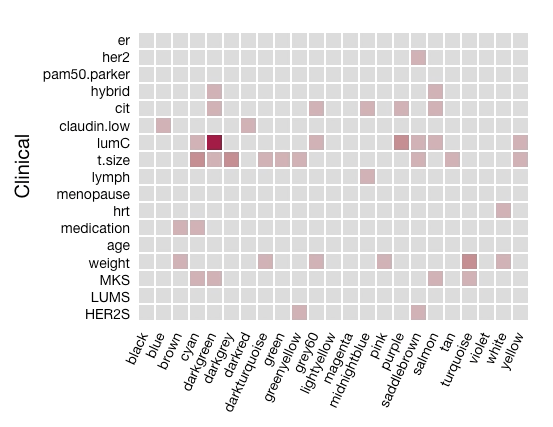
\includegraphics[width=2.5in]{figures/clinical-comp.png}
\label{fig_second_case}
\end{figure} 


\begin{figure*}[h!]
\centering
\caption{MIxT module overview page. The screenshot show the user interface for
exploring a single module. It consists of three panels. The top left panel
contains the gene expression heatmap. The top right panel contains a table of
the genes found in the module. The bottom panel contains the results of gene
overlap analyses from the module genes and known gene sets from MSigDB.}
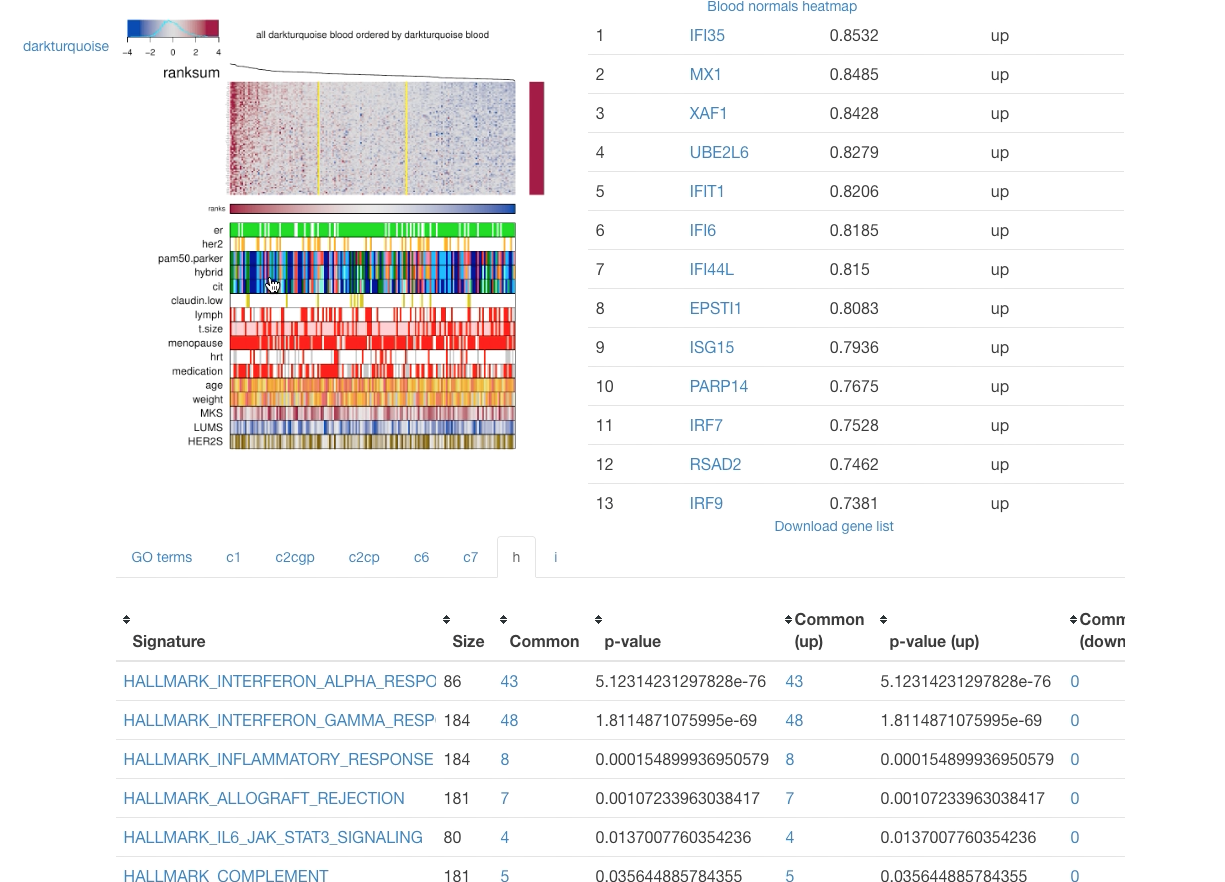
\includegraphics[width=0.8\textwidth]{figures/module.png}
\label{fig_first_case}
\end{figure*} 

\subsection*{Evaluation} 
We evaluate the performance of the services by running a set of benchmarks. To
evaluate the database service we measure the query time for retrieving
information about a specific gene with and without caching. This illustrates how
we can improve performance in an application by using a database service rather
than accessing the database directly. We also measure storage requirements for
the caching mechanism to show that it does not require a large storage capacity.
To show that it scales we show the query time for 1, 10, 100, and 1000
concurrent requests.

We evaluate the compute service by running a small example benchmark. The
benchmark consists of two operations: first generate a
set of numbers, then plot them and return the resulting visualization. We show
that the latency is low enough to use it in an interactive application. To show
that it performs under heavy load we perform the same operations using 1, 10,
100, and 1000 concurrent requests. We use two \emph{c4.large} instances on AWS
EC2\footnote{See \url{aws.amazon.com/ec2/instance-types} for more
information} running the Kvik compute service and OpenCPU base docker
containers. The servers have caching disabled. 

We first measure the total time to generate the numbers and generate the plot.
From 100 runs we measured the mean execution time for both the compute service
in Kvik and the OpenCPU. Using Kvik the mean execution time os 274ms while
OpenCPU uses 506ms. We then investigate the throughput for usage patterns with
1, 10, 100, and 1000 parallel connections. 

time to complete the benchmark when
using 1, 10, 100 or 1000 parallel connections. 

Table 

TODO: INSERT NUMBERS
